\documentclass[sigconf]{acmart}

\AtBeginDocument{%
  \providecommand\BibTeX{{%
    \normalfont B\kern-0.5em{\scshape i\kern-0.25em b}\kern-0.8em\TeX}}}

\setcopyright{acmcopyright}
\copyrightyear{2019}
\acmYear{2019}
\acmDOI{10.1145/123456789}

%% These commands are for a PROCEEDINGS abstract or paper.
\acmConference[SOSR '20]{SOSR '20}{March 2020}{San Jose, CA}
\acmBooktitle{SOSR '20,
  March 2020, San Jose, CA}
\acmPrice{15.00}
\acmISBN{978-1-4503-9999-9/20/06}


%\usepackage{cite}
\usepackage{amsmath,amssymb,amsfonts,amsthm}
\usepackage{algorithmic}
\usepackage{graphicx}
\usepackage{textcomp}
\usepackage{xcolor}
\usepackage{tikz}


%%%%futher packages
\usepackage{amsmath,amssymb,array,color,colortbl,graphicx,multirow}
%\usepackage{microtype}
\usepackage{comment}
%\usepackage{algorithm2e}
\usepackage{comment}
\usepackage{listings,color}
\usepackage{verbatim}
\usepackage{multirow}
\usepackage{listings}
\usepackage{framed,color}
\usepackage{balance}
\usepackage{url}
\usepackage{subfig}
\usepackage[ruled,vlined,linesnumbered,]{algorithm2e}


%%%%%%%%%%%%%%%%%%%%%%%%%%%%%%%TIKZ%%%%%%%%%%%%%%%%%%%%%%%%%%
\usetikzlibrary{calc}
\usetikzlibrary{chains}
\usetikzlibrary{patterns}
\usetikzlibrary{decorations.pathreplacing}
\usetikzlibrary{er}
\usetikzlibrary{shapes}
\usetikzlibrary{shapes.multipart}
\usetikzlibrary{arrows}
\tikzset{markovstate/.style={shape=circle,draw=black,align=center,inner sep=0,minimum width=7mm}}
\tikzset{markovedge/.style={-latex}}
%\tikzset{label/.style={}}
\tikzset{pkt/.style={draw,rectangle,fill=gray!15,minimum height=25pt,align=center,font=\footnotesize}}
\tikzset{pktlen/.style={above=-2pt,font=\scriptsize}}
\newcommand{\out}{\texttt{out}}
\newcommand{\inn}{\texttt{in}}
\newcommand{\dist}{\emph{dist}}
\renewcommand{\vec}[1]{\mathbf{#1}}
\definecolor{mycolor}{RGB}{0,200,100}
%%%%%%%%%%%%%%%%%%%%%%%%%%%%%%%TIKZ%%%%%%%%%%%%%%%%%%%%%%%%%%

\newcommand{\E}{\mathcal{E}}  % configurable links
\newcommand{\Lminmax}{L_{\text{min-max}}}  % configurable links

\newcommand\stefan[1]{\color{blue}\textbf{\\ Stefan: #1}\\\color{black}}
\newcommand\klaus[1]{\color{olive}\textbf{Klaus: #1}\color{black}}
\newcommand\wenkai[1]{\color{green}\textbf{Wenkai: #1}\color{black}}
\newcommand\david[1]{\color{green}\textbf{David: #1}\color{black}}
\newcommand\todo[1]{\color{red}\textbf{#1}\color{black}}


\makeatletter
\renewcommand{\SetKwInOut}[2]{%
	\sbox\algocf@inoutbox{\KwSty{#2\algocf@typo:}}%
	\expandafter\ifx\csname InOutSizeDefined\endcsname\relax% if first time used
	\newcommand\InOutSizeDefined{}\setlength{\inoutsize}{\wd\algocf@inoutbox}%
	\sbox\algocf@inoutbox{\parbox[t]{\inoutsize}{\KwSty{#2\algocf@typo\hfill:}}~}\setlength{\inoutindent}{0em}%{\wd\algocf@inoutbox}% <------------
	\else% else keep the larger dimension
	\ifdim\wd\algocf@inoutbox>\inoutsize%
	\setlength{\inoutsize}{\wd\algocf@inoutbox}%
	\sbox\algocf@inoutbox{\parbox[t]{\inoutsize}{\KwSty{#2\algocf@typo\hfill:}}~}\setlength{\inoutindent}{0em}%{\wd\algocf@inoutbox}% <------------------
	\fi%
	\fi% the dimension of the box is now defined.
	\algocf@newcommand{#1}[1]{%
		\ifthenelse{\boolean{algocf@hanginginout}}{\relax}{\algocf@seteveryparhanging{\relax}}%
		\ifthenelse{\boolean{algocf@inoutnumbered}}{\relax}{\algocf@seteveryparnl{\relax}}%
		{\let\\\algocf@newinout\hangindent=\inoutindent\hangafter=1\parbox[t]{\inoutsize}{\KwSty{#2\algocf@typo\hfill:}}~##1\par}
		\algocf@linesnumbered% reset the numbering of the lines
		\ifthenelse{\boolean{algocf@hanginginout}}{\relax}{\algocf@reseteveryparhanging}%
}}%
\makeatother

%%
%% Submission ID.
%% Use this when submitting an article to a sponsored event. You'll
%% receive a unique submission ID from the organizers
%% of the event, and this ID should be used as the parameter to this command.
%%\acmSubmissionID{123-A56-BU3}

%%
%% The majority of ACM publications use numbered citations and
%% references.  The command \citestyle{authoryear} switches to the
%% "author year" style.
%%
%% If you are preparing content for an event
%% sponsored by ACM SIGGRAPH, you must use the "author year" style of
%% citations and references.
%% Uncommenting
%% the next command will enable that style.
%%\citestyle{acmauthoryear}

%%
%% end of the preamble, start of the body of the document source.
\begin{document}

%%
%% The "title" command has an optional parameter,
%% allowing the author to define a "short title" to be used in page headers.
\title[Load-Optimization in Reconfigurable Networks: Algorithms and Complexity of Flow Routing]{Load-Optimization in Reconfigurable Networks:\\ Algorithms and Complexity of Flow Routing}

\title[When You Wish Upon a Star: Load-Optimal Routing in Programmable Topologies]{When You Wish Upon a Star:\\ Load-Optimal Routing in  Programmable Topologies} 

%%
%% The "author" command and its associated commands are used to define
%% the authors and their affiliations.
%% Of note is the shared affiliation of the first two authors, and the
%% "authornote" and "authornotemark" commands
%% used to denote shared contribution to the research.

\author{Submission \#47}
\affiliation{6 pages, plus references} % \klaus{we need a new title}}

%\settopmatter{printacmref=false}

\begin{comment}
\author{Wenkai Dai}
\affiliation{%
  \institution{University of Vienna}
  \department{Faculty of Computer Science}
  \city{Vienna}
  \country{Austria}
}
\email{wenkai.dai@univie.ac.at}


\author{Klaus-Tycho Foerster}
\affiliation{%
	\institution{University of Vienna}
	 \department{Faculty of Computer Science}
	\city{Vienna}
	\country{Austria}
}
\email{klaus-tycho.foerster@univie.ac.at}

\author{David Fuchssteiner}
\affiliation{%
	\institution{University of Vienna}
	\department{Faculty of Computer Science}
	\city{Vienna}
	\country{Austria}
}
\email{david.alexander.fuchssteiner@univie.ac.at}

\author{Stefan Schmid}
\affiliation{%
	\institution{University of Vienna}
	  \department{Faculty of Computer Science}
	\city{Vienna}
	\country{Austria}
}
\email{stefan_schmid@univie.ac.at}
\end{comment}

%%
%% By default, the full list of authors will be used in the page
%% headers. Often, this list is too long, and will overlap
%% other information printed in the page headers. This command allows
%% the author to define a more concise list
%% of authors' names for this purpose.
%\renewcommand{\shortauthors}{Trovato and Tobin, et al.}

%%
%% The abstract is a short summary of the work to be presented in the
%% article.



\begin{abstract}
Emerging reconfigurable data centers introduce unprecedented flexibility 
in how the physical layer can be programmed to adapt to current traffic demands.
These programmable topologies are commonly hybrid, consisting of static and reconfigurable links, 
enabled by e.g., an Optical Circuit Switch (OCS) combined with electrical packet switching.
Even though prior works have showcased the practical benefits of hybrid networks, 
several crucial performance aspects are not well understood.
For example, many systems do not jointly optimize both hybrid network parts, leaving money on the table.
In this paper we initiate the algorithmic study of efficient cross-layer optimization techniques to route flows efficiently in such hybrid networks, focusing on the most fundamental performance metric of link load.
The complexity of reconfiguration mechanisms in this space is unexplored at large, especially for the following cross-layer network-design problem: Given a hybrid network and a traffic matrix, jointly optimize the physical layer and the corresponding flow routing in order to minimize the maximum load among links.
A topological complexity classification of the problem reveals that already trees with two layers of packet switches are intractable, whereas networks with a single packet switch (also known as \emph{star} networks) can always be handled efficiently.
Moreover, we prove that submodularity does not hold in these settings, i.e., common approximation ideas cannot be applied to multi-layer trees.
Lastly, we perform evaluations in hybrid networks where the static network follows the abstract big switch model.
We show that our algorithmic insights significantly improve the network load-balance in comparison to the state of the art, based on real-world data center traces from Facebook.
\end{abstract}



%%
%% The code below is generated by the tool at http://dl.acm.org/ccs.cfm.
%% Please copy and paste the code instead of the example below.
%%
\begin{CCSXML}
<ccs2012>
<concept>
<concept_id>10003033.10003034</concept_id>
<concept_desc>Networks~Network architectures</concept_desc>
<concept_significance>500</concept_significance>
</concept>
<concept>
<concept_id>10003752.10003809</concept_id>
<concept_desc>Theory of computation~Design and analysis of algorithms</concept_desc>
<concept_significance>500</concept_significance>
</concept>
</ccs2012>
\end{CCSXML}

\ccsdesc[500]{Networks~Network architectures}
\ccsdesc[500]{Theory of computation~Design and analysis of algorithms}


%%
%% Keywords. The author(s) should pick words that accurately describe
%% the work being presented. Separate the keywords with commas.
%\keywords{datasets, neural networks, gaze detection, text tagging}
\keywords{programmable topologies, optical networks, algorithms, complexity}

%%
%% This command processes the author and affiliation and title
%% information and builds the first part of the formatted document.
\settopmatter{printfolios=true}
\maketitle

\section{Introduction}\label{sec:intro}
%
Data centers are a critical infrastructure of today's societies, empowering everyday life in aspects such as business, health, industry, but also science and social interactions.
%
With the rise of related data-intensive workloads as generated by machine learning, artificial intelligence, and the distributed processing of big data in general, data center traffic is growing at explosive scale~\cite{DBLP:journals/cacm/SinghOAAABBDFGK16,networking2016cisco}.
%
Much of this traffic is internal to data centers, evoking considerable research interest in data center design problems~\cite{DBLP:journals/comsur/XiaZWX17,DBLP:journals/comsur/Noormohammadpour18}.
%

%
However, electrical chips are unlikely to deliver sufficient performance for next-generation networks, and in turn we must rely on programmable optical topologies for increased bandwidth, connectivity and power-efficiency.
%
Herein the emergence of a \emph{programmable physical layer}, empowered by optical circuit switches~\cite{helios,cthrough,DBLP:journals/comsur/KachrisT12}, free-space optics~\cite{projector,Hamedazimi2014}, or beamformed wireless~\cite{augmenting,DBLP:journals/comsur/HamzaDA16}, steered by e.g.\ Software-Defined Networking~\cite{alsmadi2017systematic}, leads to exciting new possibilities---analogously to the progress enabled by programmable control and data planes in SDNs~\cite{DBLP:conf/hpsr/BifulcoR18,DBLP:journals/pieee/KreutzRVRAU15,DBLP:journals/ccr/FeamsterRZ14}. 
%, as ''\textit{the 'big-switch' illusion of full bisection bandwidth} [...] \textit{is increasingly cost prohibitive and likely soon infeasible~\cite{DBLP:conf/hotnets/MelletteSP16}}''~\cite{opera}.
 %In other words, 
 %
 
% 
Extensive  works in the past have already shown significant benefits of such reconfigurable data center networks~\cite{DBLP:journals/sigact/FoersterS19}, but the underlying complexity is not well understood~\cite{DBLP:journals/ccr/AvinS18}.
%
For example, many works do not jointly optimize the hybrid network, but rather treat the packet switched part as an afterthought~\cite{DBLP:conf/ancs/FoersterGS18}.

%For example, many works artificially restrict their flow routing policies to be segregated between programmable and static network parts, aiming to place elephant flows on reconfigurable links~\cite{DBLP:conf/ancs/FoersterGS18}.
%

%
Whereas some general algorithmic results exist w.r.t.\ latency~\cite{projector,DBLP:journals/ccr/FoersterPS19} or specific traffic patterns~\cite{eclipse-journal,DBLP:conf/infocom/Avin0019}, complexity questions of network-design for the objective of load-optimization are mostly uncharted.
%
At the same time, link load is a most central performance metric~\cite{DBLP:conf/conext/CaoXYGLYZWXM13,DBLP:journals/ton/SridharanGD05}, and flow routing in traditional networks has been investigated for decades already~\cite{DBLP:books/daglib/0069809}
%


%
Our paper is thus motivated by the desire to take the first steps towards fundamentally understanding the network-design problem for load-optimization, which jointly considers flow routing and physical layer programmability in data center networks.

\smallskip
%\subsection{Contributions}\label{subsec:contributions}
\noindent\textbf{Contributions.}
This paper initiates the network-design study of load-optimization in reconfigurable networks, leveraging the flexibility of emerging programmable physical layers for flow routing.
%We investigate multiple problem dimensions, from splittable to unsplittable flows, to fully flexible (non-segregated) versus segregated routing policies.
%
Our results not only include efficient algorithms and complexity characterizations, but also simulations on real-world workloads:
\begin{enumerate}
    \item \emph{Complexity:} We prove strong NP-hardness already on trees of depth $\geq 2$, even if the demands are just between leaf nodes. Moreover, the problem setting is not submodular.
    %for non-segregated and segregated routing on trees of any depth greater or equal than two, for both un-/splittable flow models. Moreover, all four problem settings are not submodular.
    \item \emph{Algorithms:} In turn, we present a new polynomial-time algorithm on networks where the static network can be abstracted as a single packet switch, i.e., \emph{star} networks. 
    %While the non-segregated case of unsplittable flows is weakly NP-hard, we still obtain tractability for non-exponential flow sizes. Moreover, we design several efficient general heuristics.
    \item \emph{Evaluations:} Our workload-driven simulations (using Facebook traces) show that our algorithmic insights significantly outperform state-of-the-art methods, reducing the maximum load by nearly up to 50\%, at similar computation times.
\end{enumerate}

%\subsection{Overview}\label{subsec:overview}
%
\noindent\textbf{Overview.}
We start with a formal model in \S\ref{sec:model}, followed by intractability  and submodularity insights in \S\ref{sec:combined}. 
%
We then present our algorithmic results and bounds in \S\ref{sec:star}, which we in turn evaluate in~\S\ref{sec:eval}.
%
Lastly, we discuss the related work in \S\ref{sec:related} and conclude in \S\ref{sec:conclusion}.


\section{Model}\label{sec:model} % and Preliminary Definitions
%\subsection{Model Assumptions}
\noindent\textbf{Network model.} Let  $N=(V,E,S,\E)$ be a \emph{hybrid} network \cite{solstice,eclipse} connecting the $n$ nodes $V=\{v_1,\dots,v_n\}$ (e.g., top-of-the-rack switches), using static links $E$ (usually realized by electrical packet switches), while $N$ contains a set of reconfigurable (usually optical) links $\E$.
In order to enhance $N$, the  (optical) circuit switch $S$ can dynamically select a subset of the reconfigurable links $M\subseteq \E$, which must induce \emph{a matching}.
Without loss of generality, we assume that all links have unlimited capacities and are undirected (bidirectional), where our objective will be to minimize their load.
%\todo{Without loss of generality, we assume that a reconfigurable link $e\in \E$ is available for any two nodes $u,v \in V$,}\  and all of static links $E$ and reconfigurable links $\E$ are undirected (bidrectional) links with unlimited capacities.



%However, after a reconfigurable link $(u,v)\in \E$ being implemented by $S$, two endpoints nodes $u$ and $v$ cannot be connected by any other reconfigurable links.  Thus, only a subset of reconfigurable links that induces (a \emph{matching}) $M \subset\E$ can be implemented by a reconfigurable switch $S$ to enhance $N$.

\noindent\textbf{Reconfigured Network.}
We say that a hybrid network $N$ is \emph{reconfigured}
by a reconfigurable switch $S$ if some reconfigurable links $M\subseteq \E$ that induce a matching, are \emph{configured} (implemented) by $S$ in the network $N$. The set of configured links $M$ is called \emph{a reconfiguration} of $N$, and the enhanced network obtained by integrating the configured links $M$ (a matching) with the static links $E$ of the original network $N$ is called a \emph{reconfigured network} $N(M)$. Note that the hybrid network $N$ consisting of only static links before  reconfiguration is also a reconfigured network with $N=N(\emptyset)$. 

\noindent\textbf{Generality.}
Our results also apply to non-optical switches and links, as long as they match the theoretical properties described in the model.
As such, we will only talk about reconfigurable switches and reconfigurable links, simply implying any appropriate technology that matches our model.


\noindent\textbf{Traffic and Routing.} 
The resulting network should serve a certain 
communication pattern, represented as a $|V| \times |V|$ 
communication matrix $D:=\left( d_{ij}\right)_{|V| \times |V|} $
(\emph{demands}) with non-negative real-valued entries. 
An entry $d_{ij}\in \mathbb{R}_{\geq 0}$ represents the traffic load (frequency) or a demand
from the node $v_i$ to the node $v_j$. With slight abuse of notation,  let $D(v_i,v_j)$ also denote demands from $v_i$ to $v_j$ hereafter.
We assume that each demand has to be routed along a simple path, either along the static or the reconfigurable network parts~\cite{helios,cthrough}.
%\vspace{0.1cm}

%\noindent\textbf{Routing model.} \klaus{I will update this}In traditional multi-commodity flow problems, \emph{unsplittable} flows require that all flows of a demand for each commodity must be sent along a single path, while \emph{splittable} flows does not restrict the number of paths used for conveying flows for each commodity; For a reconfigured network, segregated routing  forbids configured links to convey flows that are also transmitted on static links, but non-segregated routing admits configured links to be used as shortcuts for flows along static links. In this paper, we only consider  the  \emph{Unsplittable \& Segregated (US)} routing model in reconfigured networks.
%\klaus{let us not use the term US anymore, we only have one routing model}


\noindent\textbf{Load Optimization.} 
%
For a reconfigured network $N(M)$ and demands $D$, let  $f:E\cup M\mapsto \mathbb{R}^+$ be \emph{a feasible flow} to serve demands $D$ in $N(M)$;
%
Note that every demand in $D$ can be served in $N(M)$ due to the (theoretically) unlimited capacities of links. 
%
Then, \emph{the maximum load} of a feasible flow $f$ is defined as ${L_\textnormal{max}(f)}:=\max\{f(e): e\in E\cup M\}$, and there must be \emph{an optimal flow} $f_{\text{opt}}$ such that its maximum load is minimized in terms of all feasible flows in $N(M)$.
%
Such an optimal flow  is called \emph{a load-optimization flow} in $N(M)$.
%
For a reconfigured network $N(M)$, with slight abuse of notation, we use $f^{M}_{\text{opt}}$ to denote an arbitrary load-optimization flow in $N(M)$  and define a function $L_{\text{min-max}}\left(N(M) \right):=L_{max}\left(f^{M}_{\text{opt}}\right)$.
%
A load-optimization flow is a special case of a load-balancing (a minimized maximum load) flow problem in multi-commodity flow networks, where each link has the same capacity.
%
%In other words, the existence of a load-optimization flow with maximum load $L_{max}$ implies feasible routing in a network with link capacities of $L_{max}$.




\noindent\textbf{Load-Optimization Reconfiguration Problem.} 
Given a hybrid network $N$ and demands $D$, the \emph{load-optimization reconfiguration problem} is to get \emph{an  optimal reconfiguration} by selecting a matching $M\subseteq \E$ from all reconfigurable links $\E$ to generate \emph{an optimally reconfigured network} $N(M)$ such that $L_{\text{min-max}}\left(N(M) \right)$ is minimized for all possible reconfigurations $M_i\subseteq\E$ of $N$.
%
We also need to find a load-optimization flow  for the optimally reconfigured network. % $N(M)$. %The US-load-optimization reconfiguration problem is also abbreviated as \emph{US-reconfiguration problem}.



%\subsection{\todo{Temporary} Preliminary Definitions}
%We also briefly introduce some problems as follows, which will be referenced in our later proofs.%\cite{Garey:1979:CIG:578533}
%\todo{please state that we made this problem up}



%\begin{definition}[\textsc{Min-Load Reconfigured Triangle Multicommodity Flow (MRTMF)}]
%	Given a complete graph $G=(V,E)$, where $V=\{v_i,v_j,v_c\}$, Demands $D$, and $(v_i,v_j)$ is a configured link, to find a multicommodity flow $f$ under flowing models of  US,  SS, and SN respectively such that $\max\{f(e):e\in E\}$ is minimized (the minimized max flow value is called the min-load and  denoted by  $\text{min}_{i,j}$).\label{def:MRTMF}
%\end{definition}

\section{Complexity}\label{sec:combined}
We start our investigation with a detailed complexity discussion.
To this end, we show the reconfiguration problem to be NP-hard in \S\ref{sec:complexity} and that it is non-submodular in \S\ref{sec:sub}.

\subsection{Intractability}\label{sec:complexity}
In this section, we show that  a static tree network with the height of two already implies intractability, even if just the leaf nodes have demands.
%To prove the NP-hardness in a formal way, we first define the corresponding decision problem of reconfiguration:

%\noindent\textbf{Decision Problem of Reconfiguration} The decision problem of a reconfiguration problem is to decide that for a given hybrid network $N$, demands $D$, and a threshold $\lambda$, if we can find a configuration (a matching) $M$ such that  the configured network $N(M)$ has $L_{\text{min-max}}\left(N(M) \right)\leq \lambda$ to serve $D$?

\begin{theorem}
	The reconfiguration problem is strongly NP-hard when the given hybrid network $N$ is a tree of the height $h\ge 2$, where demands just occur between leaf nodes. \label{thm:1}
\end{theorem}

Our proof will be by a reduction from \textsc{$3$-Partition}, where the intractability arguments rely on the load-optimization of the interior tree links. We defer the proof details due to space constraints.

\subsection{Non-Submodularity}\label{sec:sub}
We recall the definition of submodularity~\cite{Goemans:2009:ASF:1496770.1496829}: 
%
A function $f:2^{B}\mapsto \mathbb{R}$, where $2^{B}$ is a power set of a finite set $B$, is  submodular if it satisfies that for every $X,Y \subseteq B$ with $X\subseteq Y$ and every $x\in B \setminus Y$,
%
\[ f\left(X\cup\left\{x\right\}\right)-f\left(X \right)  \ge f\left(Y\cup\left\{x\right\}\right)-f\left(Y\right)\,.   \]
The submodularity of objective functions plays an important role in approximating optimization problems~\cite{Vazirani:2001:AA:500776}.  
%
In this section, we investigate the submodularity of the objective function $\Omega$ of the reconfiguration problem. 
%
To this end, we also consider the submodularity of another objective function $\Phi$ that maximizes the gap of the minimized maximum load between the original network and the reconfigured network. 
%
We will show that both functions $\Omega$ and $\Phi$ are not submodular functions. 
%
To prove the functions to be not submodular, we present special instances as counter-examples. 
%
\begin{theorem}
	For the reconfiguration problem, the objective function $\Pi$, that minimizes the maximum load of the reconfigured network $N(M)$ for reconfigurations $M$, is not submodular. 
\end{theorem}
\begin{proof}
	For a hybrid network $N=(V,E,S,\E,D)$, we define the set of nodes $V=U\cup Q$, where $U=\{u_i:i=1,2,3\}$ and $Q=\{q_i:i=1,2,3\}$. For static links $E$, we have  six static links: $(u_1,u_2), (u_1,u_3)\in E$, $(q_1,q_2),(q_1,q_3)\in E$, and $(u_2,q_2),(u_3,q_3)\in E$.  For each $i\in \{1,2,3\}$, there is  a reconfigurable link $(u_i,q_i)\in \E$. We have the following demands: $D(q_3,u_3)=3$, $D(u_2,q_2)=3$, $D(q_2,u_2)=3$ and $D(u_1,q_1)=3$.  Let our objective function $\Pi: 2^\E\mapsto \mathbb{R}_{\ge0}$ be a function defined by an equation $\Pi\left(M\right)=L_{\textnormal{min-max}}\left(N(M)\right)$, where  $M\in 2^\E$ is a reconfiguration (matching). Recall the definition of submodularity. We set $X=\{(u_2,q_2)\}\subseteq\E$, $Y=\{(u_1,q_1),(u_2,q_2)\}\subseteq\E$ and $x=(u_3,q_3)\in\E$. By our routing rules,  we can easily decide $L_{\text{min-max}}\left(N \right)=6$, $\Pi\left(X \cup\{x\}\right)=3$, $\Pi\left(X\right)=6$, $\Pi\left(Y\cup\{x\}\right)=3$, and $\Pi\left(Y\right)=3$. Thus, the inequality~\eqref{eq:nonsub_pi} shows that the function $\Pi$ is not submodular. 
	\begin{equation}
	\Phi\left(X\cup\left\{x\right\}\right)-\Phi\left(X \right)=-3  < \Phi\left(Y\cup\left\{x\right\}\right)-\Phi\left(Y\right)=0\, \label{eq:nonsub_pi}
	\end{equation}
\end{proof}

\begin{theorem}
For the reconfiguration problem, the objective function $\Phi$, that maximizes the gap of the minimum maximum loads between the given hybrid network $N$ and the reconfigured network $N(M)$ for all reconfigurations $M$ of $N$, is not submodular. 
\end{theorem}
\begin{proof}
	For a hybrid network $N=(V,E,S,\E,D)$, we define the set of nodes $V=U\cup Q$, where $U=\{u_i:i=1,2,3\}$ and $Q=\{q_i:i=1,2,3\}$, and for each $i\in \{1,2,3\}$, we set a static link $(u_i,q_i)\in E$ and a reconfigurable link $(u_i,q_i)\in \E$, and two demands $D(u_i,q_i)=3$ and $D(q_i,u_i)=3$. Let our objective function $\Phi: 2^\E\mapsto \mathbb{R}_{\ge0}$ be a function defined by an equation $\Phi\left(M\right)=\phi-L_{\textnormal{min-max}}\left(N(M)\right)$, where  a reconfiguration (matching) $M\in 2^\E$ and   $\phi=L_{\textnormal{min-max}}\left(N\right)$. Recall the definition of submodularity. We set $X=\{(u_1,q_1)\}$, $Y=\{(u_1,q_1),(u_2,q_2)\}$ and $x=(u_3,q_3)$. For our routing rules,  we can easily decide $L_{\text{min-max}}\left(N \right)=6$, $\Phi\left(X \cup\{x\}\right)=\phi-6$, $\Phi\left(X\right)=\phi-6$, $\Phi\left(Y\cup\{x\}\right)=\phi-3$, and $\Phi\left(Y\right)=\phi-6$. Thus, the inequality~\eqref{eq:nonsub_phi} shows that the function $\Phi$ is not submodular. 
	
	\begin{equation}
\left(\Phi\left(X\cup\left\{x\right\}\right)-\Phi\left(X \right)=0\right)  < \left(\Phi\left(Y\cup\left\{x\right\}\right)-\Phi\left(Y\right)=3\right)\, \label{eq:nonsub_phi} 
	\end{equation}
\end{proof}
\wenkai{you remove the inequality and say phi is not submodular to save space}
\section{Optimality for Star Networks}\label{sec:star}

\begin{figure}[b]
	\centering
	\scalebox{0.6}{
		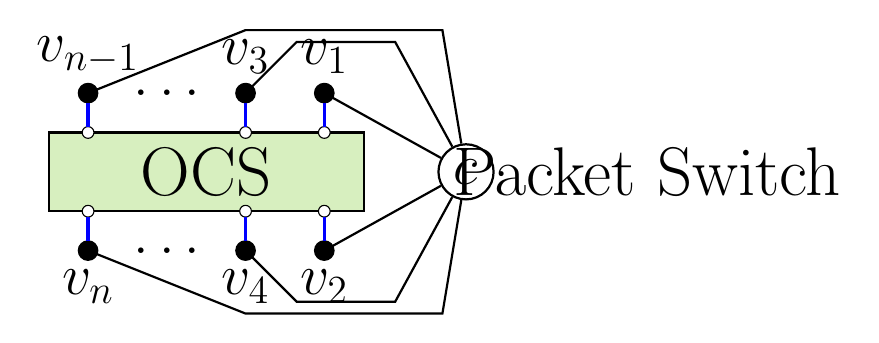
\begin{tikzpicture}
		
	%	\draw [thick, dotted] (1.5,-0.5) rectangle (4.5,2.5);
		
		%\draw [thick, dotted] (5.5,-0.5) rectangle (8.5,2.5);
		
		\definecolor{dunkelgruen}{RGB}{122,202,42}
	\draw[draw=black,  thick, fill=dunkelgruen!30] (-3.5,0.5) rectangle node{\Huge OCS} ++(4,1);
	%\draw[draw=black,  thick, fill=dunkelgruen!30] (-3.5,0.5) rectangle node{\Huge OCS} ++(4,1);
%		\draw[draw=black, thick, fill=dunkelgruen] (7,-0.5) rectangle ++(1.0,3.0);
		
\draw (0,2) node[circle,draw, fill=black, outer sep=0pt,inner sep=2.5pt, minimum size=5pt,  label=above:{\huge $v_1$}] (v1) {} ;

\draw (0,0) node[circle,draw, fill=black, outer sep=0pt,inner sep=2.5pt, minimum size=5pt, label=below:{\huge $v_2$}] (v2) {} ;

\draw (-1,2) node[circle,draw, fill=black, outer sep=0pt,inner sep=2.5pt, minimum size=5pt,  label=above:{\huge $v_3$}] (v3) {} ;

\draw (-1,0) node[circle,draw, fill=black, outer sep=0pt,inner sep=2.5pt, minimum size=5pt, label=below:{\huge $v_4$}] (v4) {} ;

\draw (-3,2) node[circle,draw, fill=black, outer sep=0pt,inner sep=2.5pt, minimum size=5pt,  label=above:{\huge $v_{n-1}$}] (vn-1) {} ;

\draw (-3,0) node[circle,draw, fill=black, outer sep=0pt,inner sep=2.5pt, minimum size=5pt, label=below:{\huge $v_{n}$}] (vn) {} ;

\draw (0,1.5) node[circle,draw, fill=white!50, outer sep=0pt,inner sep=1.5pt, minimum size=3pt, ] (D1) {} ;

\draw (v2)+(0,0.5) node[circle,draw, fill=white!50, outer sep=0pt,inner sep=1.5pt, minimum size=3pt, ] (D2) {} ;

\draw (v3)+(0,-0.5) node[circle,draw, fill=white!50, outer sep=0pt,inner sep=1.5pt, minimum size=3pt, ] (D3) {} ;

\draw (v4)+(0,0.5) node[circle,draw, fill=white!50, outer sep=0pt,inner sep=1.5pt, minimum size=3pt, ] (D4) {} ;

\draw (vn-1)+(0,-0.5) node[circle,draw, fill=white!50, outer sep=0pt,inner sep=1.5pt, minimum size=3pt, ] (Dn-1) {} ;
\draw (vn)+(0,0.5) node[circle,draw, fill=white!50, outer sep=0pt,inner sep=1.5pt, minimum size=3pt, ] (Dn) {} ;

\node at (4.1,1) {\Huge Packet Switch};
    
    
    \node at ($(v3)!.5!(vn-1)$) {\huge$\boldmath{\ldots}$};
    
     \node at ($(v4)!.5!(vn)$) {\huge$\boldmath{\ldots}$};



		\node [markovstate,thick] (c) at (1.8,1) {\huge$c$};
		
				\draw [thick] (c) to (v1);
				\draw [thick] (c) to (v2);
				
				

				
				\draw [very thick,blue] (v1) to (D1);
				\draw [very thick, blue] (v2) to (D2);
				
				\draw [very thick,blue] (v3) to (D3);
				\draw [very thick, blue] (v4) to (D4);
				
				\draw [very thick,blue] (vn-1) to (Dn-1);
				\draw [very thick, blue] (vn) to (Dn);
				
				
				\draw [ thick,black] (v3) -- +(0.65,0.65)-- (0.9,2.65)--(c);
				
				\draw [ thick,black] (v4) -- +(0.65,-0.65)-- (0.9,-0.65)--(c);
				
				
								
				\draw [ thick,black] (vn-1) -- +(2,0.8)-- (1.5,2.8)--(c);
				
				\draw [ thick,black] (vn) -- +(2,-0.8)-- (1.5,-0.8)--(c);
			
				

		\end{tikzpicture}
	}
	\vspace{-0.1cm}
	\caption{Illustration of a hybrid star network as in~\cite[Figure 1]{eclipse}. Each of the $n$ nodes is connected to both a packet switch (denoted by $c$) and a reconfigurable swith (e.g.\ an OCS), where the latter provides a matching of the nodes.
	%Topology for a Star network with  a packet switch: the center $c$, a reconfigurable switch: OCS, and $n$ leaves: $\{v_1,\ldots,v_n\}$. 
		%, where the two optical switches are identified by the surrounding dashed squares. All links without weights depicted have a weight of zero. 
	}
	\label{fig:topology}
	%\vspace{-0.2cm}
\end{figure}

As we saw in the last sections, already simple tree networks of height $\geq 2$ are intractable, and moreover the problem setting is non-submodular, not allowing for standard approximation techniques.
%

We thus turn our attention to star networks, which are represented by a packet switch connected to all nodes, see Fig.~\ref{fig:topology}.
%
Routing in star networks is straightforward (only one simple path exists for each node pair), but the addition of a circuit switch adds a large degree of freedom:
%
First, the number of possible matchings grows exponentially, and second, we have to decide for each flow which path to take as well.
%
Notwithstanding, the special structure of star networks allows us to solve the reconfiguration problem efficiently.
%

%
We structure our approach as follows.
We first introduce an auxilliary problem in \S\ref{subsec:rtm} and a constant-time triangle graph algorithm in \S\ref{subsec:triangle}, which we then leverage for our optimal algorithm in \S\ref{subsec:staralgo}.
We lastly discuss performance bounds and extensions in \S\ref{subsec:lowerupper}.

\subsection{Red-Target Matching}\label{subsec:rtm}
Later in our algorithm, we will mark nodes (in red) which need to be connected to e.g.\ the OCS in order to satisfy the load threshold.
Not all reconfigurable connections are suitable for such a task, we identify them in the next subsection.
Given such red nodes and corresponding links, the question is if the nodes can be matched accordingly, which we denote as \textsc{Red-Target Matching}:

\begin{definition}[\textsc{Red-Target Matching (RTM)}]
	Given a graph $G=(V,E)$ and a coloring $l: V\mapsto \{r,b\}$, the question is to find a matching $M$ of $G$ such that each vertex $v\in V$ with the color $l(v)=r$ is an endpoint of a link of $M$. \label{def:RTM}
\end{definition}


\begin{lemma}
	The \textsc{RTM} problem (Definition~\ref{def:RTM}) can be solved by a maximum-weight matching algorithm in polynomial time. \label{lem:RTM}
\end{lemma}
\begin{proof}
	For a given graph $G=(V,E)$, if a link $e\in E$ has  both endpoints of  color $b$ (blue), then it can be removed directly. For each link $e\in E$ having both endpoints of color $r$ (red), we set the weight $w(e)=2$, and for each link $e\in E$ that has one endpoint of color $r$, we set  $w(e)=1$. 
	%
	Let the number of red-colored vertices in $G$ be $n$. 
	%
	If we can find a matching $M$ of the weight $n$, then all of these $n$ red vertices are contained in $M$. 
	%
	There is no matching that can have a weight more than $n$, otherwise the number of red-colored vertices in $G$ are more than $n$.
	%
	Therefore, if RTM has a solution $M$ then a maximum-weight algorithm can always find a valid matching for RTM.
	%
	If the maximum-weight matching has a weight of less than $n$, then RTM has no solution. 
	%
	Lastly, a maximum-weight matching is solvable in polynomial time, e.g., by the Blossom algorithm~\cite{Edmonds1965}.
\end{proof}

\begin{algorithm}
	\SetKwInOut{Input}{Input}\SetKwInOut{Output}{Output}
	\Input{A star  $N=(V,E,S,\E)$, where $V=\{v_1,\ldots,v_n,c\}$ (the center $c$),   $E=\left\{(v_i,c): v_i\in V\setminus \{c\}\right\}$,  $\E=\left\lbrace (v_i,v_j): v_i,v_j\in V\setminus\{c\} \right\rbrace $ and demands $D$\;}
	\Output{A matching (configured links) $M$ and a load-optimization flow $f_{\text{final}}$ of $N(M)$ or ``null''\;}
	
	Find the original (unique) flow $f_{\textnormal{old}}:E\mapsto \mathbb{R}_{\ge 0}$ serving all demands $D$ on $N$ before reconfiguration\;
	Define a set $\mathcal{P}:=\emptyset$\;

	
	\For{each reconfigurable link $(v_i,v_j)\in \E$}{
        Run Algorithm~\ref{alg:delta} on $\left(N,D, f_{\textnormal{old}}, \{v_i,v_j\}\right)$ to return $f^{\textnormal{opt}}_{i,j}$  \;
		$\mathcal{P}=\mathcal{P}\bigcup \left\{\left( (v_i,v_j), L_\text{max}\left( f_{\textnormal{opt}}^{i,j}\right), f_{\textnormal{opt}}^{i,j}\right) \right\}$\;	}
	Run Algorithm~\ref{alg:determine} on the input $(N,D,f_{\textnormal{old}},\mathcal{P})$\;
	
	\eIf{Algorithm~\ref{alg:determine} returns a RTM matching $M$}
	{compute the load-optimization flow $f_{\text{final}}$ for $N(M)$ and $D$ based on $\mathcal{P}$, where $f_{\text{final}}$ can be constructed by each flows $f_{\textnormal{opt}}^{i,j}$ in $\mathcal{P}$ with $(v_i,v_j)\in M$\;
		
		\Return $M$ and $f_{\text{final}}$\;}{\Return ``null''\;}
	
	\caption{Reconfiguration for Star Networks}\label{alg:1}
\end{algorithm} 

\subsection{Selection of Suitable Reconfigurable Links}\label{subsec:triangle}
In the  star networks considered by us, reconfigurable links can be created between any pair of leaf nodes, e.g.\ via the OCS.
While we will select the  (matching) subset of links in the next subsection, we herein identify the benefit of adding specific reconfigurable links.


\begin{lemma}
Given a star network $N$ and demands $D$, let $f_{\textnormal{old}}$ be the original flow serving $D$ before reconfiguration, and for any reconfiguration $M_i$, let $f^{M_i}_{\textnormal{opt}}$ be a load-optimization flow serving $D$ in $N(M_i)$.  For each configured link $(v_i,v_j)\in M_i$, let $f_{\textnormal{opt}}^{i,j}$ be a flow returned by Algorithm~\ref{alg:delta} and $E_{\Delta_{i,j}}:=\left\{(v_i,v_j), (v_i,c), (v_j,c)\right\}$, where $c$ is the central node,  then we have
\begin{equation}
    \max\left\{f^{M_i}_{\textnormal{opt}}\left(e\right): e\in E_{\Delta_{i,j}}\right\} \ge \max\left\{f_{\textnormal{opt}}^{i,j}\left(e\right): e\in E_{\Delta_{i,j}}\right\}\; ; \label{eq:delta}
\end{equation}
Moreover,  Algorithm~\ref{alg:delta} runs in constant time for each triangle. \label{lem:delta}
\end{lemma}
\begin{proof}
%Recall the definition of the routing model, and then 
In triangle $\{v_i,v_j,c\}$, after removing flows for $D(v_i,v_j)$ and $D(v_j,v_i)$ in $f_{\textnormal{opt}}^{i,j}$ and $f^{M_i}_{\textnormal{opt}}$ respectively, the remaining flows on static links $(v_i,c)$ and $(v_j,c)$ for $f_{\textnormal{opt}}^{i,j}$ and $f^{M_i}_{\textnormal{opt}}$ must be identical and fixed, which are also tractable in the original flow $f_{\textnormal{old}}$ since the configured link $(v_i,v_j)$ can only serve for $D(v_i,v_j)$ and $D(v_j,v_i)$. In Algorithm~\ref{alg:delta}, the flows for $D(v_i,v_j)$ and $D(v_j,v_i)$ in $f_{\textnormal{opt}}^{i,j}$  are designed to minimize the maximum load of  links of $E_{\Delta_{i,j}}$. Thus, the equation~\eqref{eq:delta} holds.
%
In Algorithm~\ref{alg:delta}, the removal of the corresponding flows for demands $D(v_i,v_j)$ and $D(v_j,v_i)$ (Line~$2$) can be done in  constant time, since these flows are only on the unique path $(v_i,c,v_j)$ before the reconfiguration. For the considered routing model, there are only four ways to serve $D(v_i,v_j)$ and $D(v_j,v_i)$: 1) both on the reconfigured link $(v_i,v_j)$, 2) both on the path (static links) $(v_i,c,v_j)$, and 3) $D(v_i,v_j)$ sent on $(v_i,v_j)$ while $D(v_j,v_i)$ going on static links, etc. Thus, the load-optimization flow $f_{\textnormal{opt}}^{i,j}$ for the triangle $\{v_i,v_j,c\}$ can be determined by trying these four cases in constant time provided that flows for other demands except for $D(v_j,v_i)$ and $D(v_i,v_j)$ are fixed on $(v_i,c)$ and $(v_j,c)$.
\end{proof}
\begin{algorithm}
	\SetKwInOut{Input}{Input}\SetKwInOut{Output}{Output}
	\Input{Star $N$, demands $D$, the original flow $f_{\textnormal{old}}$ and two leaf nodes $v_i,v_j\in V\setminus\{c\}$\;}
	\Output{a load-otimization flow $f_{\textnormal{opt}}^{i,j}$ for $\{v_i,v_j, c\}$\;}
	

		Define the triangle on nodes $\{v_i,v_j,c\}$, where a configured link $\E_{i,j}=(v_i,v_j)$ and static links $E_{i,j}=\{(v_i,c), (v_j,c)\}$ \;
	    Remove  the corresponding flows for demands $D(v_i,v_j)$ and $D(v_j,v_i)$ in $f_{\textnormal{old}}$ to obtain a new flow $f^{\textnormal{old}}_{i,j}:E\mapsto \mathbb{R}_{\ge 0}$  \;
        Define a flow  on the triangle $\{v_i,v_j,c\}$: $f_{\textnormal{opt}}^{i,j}: \E_{i,j}\cup E_{i,j}\mapsto\mathbb{R}_{\ge0}$ s. t., $\forall{e\in E_{i,j}}: f_{\textnormal{opt}}^{i,j}(e)= f^{\textnormal{old}}_{i,j}(e)$\;
        Based on the existing flows in $f_{\text{opt}}^{i,j}$, update $f_{\text{opt}}^{i,j}$ to be a  load-optimization flow to serve demands $D(v_i,v_j)$ and $D(v_j,v_i)$\;
		\Return the load-optimization flow $f_{\textnormal{opt}}^{i,j}$ for the triangle $\{v_i,v_j,c\}$\;
	
	\caption{Triangle Optimization}\label{alg:delta}
\end{algorithm} 

\begin{algorithm}
	\SetKwInOut{Input}{Input}\SetKwInOut{Output}{Output}
	\Input{A star $N$, where nodes $V=\{v_1,\ldots,v_n,c\}$, demands $D$, the original flow $f_{\textnormal{old}}$, and a set $\mathcal{P}$ of $\frac{n(n-1)}{2}$ triples $\left( (v_i,v_j), L_\text{max}\left( f_{\textnormal{opt}}^{i,j}\right), f_{\textnormal{opt}}^{i,j}\right)$\;}
	\Output{Configured links (a matching) $M$ or ``null''\;}
	Define a set $\mathcal{S}=\emptyset$\;
	\For{each static link $\{v_i,c\}\in E$}{$\mathcal{S}=\mathcal{S}\bigcup f_{\textnormal{old}}\left( (v_i,c)\right) $, where $f_{\textnormal{old}}$ is the original flow\;}
	\For{each triple  $\left( (v_i,v_j), L_\text{max}\left( f_{\textnormal{opt}}^{i,j}\right), f_{\textnormal{opt}}^{i,j}\right)\in \mathcal{P}$}{$\mathcal{S}=\mathcal{S}\bigcup L_\text{max}\left( f_{\textnormal{opt}}^{i,j}\right)$\;}
	Sort elements  of  $\mathcal{S}$ in  ascending order, where $\mathcal{S}\subset\mathbb{R}_{\ge0}$\;
	\For{each positive element $\lambda\in \mathcal{S}$ in the sorted set $\mathcal{S}$}{

		Create a  graph $G$ on leaf nodes $V\setminus\{c\}$ without links\;
		
		\For{each static link $(v_i,c)\in E$}{\eIf{$f_{\textnormal{old}}\left((v_i,c)\right)>\lambda$}{color the corresponding $v_i\in V\setminus\{c\}$  by ``red''\;}{color the corresponding $v_i\in V\setminus\{c\}$  by ``blue''\;}}

		\For{each triple  $\left( (v_i,v_j), L_\text{max}\left( f_{\textnormal{opt}}^{i,j}\right), f_{\textnormal{opt}}^{i,j}\right) \in  \mathcal{P}$}{
		\If{$L_\text{max}\left( f_{\textnormal{opt}}^{i,j}\right)\leq \lambda$}{add a link $(v_i,v_j)$ into $G$\;}}
		
		solve RTM problem to cover all ``red'' nodes in $G$\;
		\Return  a RTM matching $M$ or ``null''\;
		
	}
	\caption{RTM Matching on Star Networks}\label{alg:determine}
\end{algorithm} 

\subsection{Solving Stars Optimally}\label{subsec:staralgo}
We now combine our previous results to optimally solve the reconfiguration problem on star networks.
For ease of notation, we define a star network as $n$ nodes connected by a single packet switch.

%, and $2)$ denote by $\textsc{MaxMatching}(\textnormal{Star}(n))$ the run time of the seminal Blossom algorithm~\cite{Edmonds1965} to compute a maximum weight matching.

%\klaus{Wenkai, please also add the runtime of the algorithm in $O$-notation}
\begin{theorem}\label{thm:opt1}
The reconfiguration problem on star networks is solved optimally by Algorithm~\ref{alg:1}.
%in a run time of $O\left( n^2+2\log_2n*\textsc{MaxMatching}(\textnormal{Star}(n))\right) $
%The US-reconfiguration problem on star networks, where reconfigurable links are only between leaf nodes,  is solved by Algorithm~\ref{alg:1} i of $O\left( n^2+2\log_2n*n^4\right) $, where $n$ is the number of leaf nodes and $O(n^4)$ occurs in computing a maximum weight matching by classic Blossom algorithm~\cite{Edmonds1965}.
\end{theorem}
\begin{proof}
Given a  hybrid star network $N=(V,E,S,\E)$, where the reconfigurable links $\E$ are only between leaf nodes, let a set of reconfigurable links (a matching) $M^{*}\subseteq \E$ be an optimal reconfiguration of $N$. 
%
For the reconfigured network $N\left( M^*\right) $, a load-optimization flow $f^{M^*}_{\text{opt}}$, where $L_{\text{max}}\left( f^{M^*}_{\text{opt}}\right) =L_{\text{min-max}}\left( N\left( M^*\right) \right)$, must exist. 
%
We define a constant value  $\lambda^*=L_{\text{max}}\left( f^{M^*}_{\text{opt}}\right)$. For the flow $f^{M^*}_{\text{opt}}$ on $N\left( M^* \right) $, there must be at least one link either $e^*\in E$ or $e^*\in M^{*}$ such that $f^{M^*}_{\text{opt}}\left( e^*\right)=\lambda^*$. When $e^*\in E$, where $e^*=\{v_i,c\}$,  if the leaf node $v_i$ of $e^*$ is not contained in any configured link of $M^*$, then the Line~$3$ of Algorithm~\ref{alg:determine} must store $\lambda^*$ in the set $\mathcal{S}$ since the flows on the static link, whose leaf node is not included in any configured link, is unchanged after reconfiguration. Now, we assume that one endpoint of $e^*$ is a leaf node included in a configured link of $M^*$, where $e^*$ can be a static link or a reconfigurable link in $M^*$. Without loss of generality, we assume $e^*$ is a link in a triangle $\{v_i,v_j,c\}$, where $(v_i,v_j)\in M^*$. By Lemma~\ref{lem:delta}, the load-optimization flow $f_{\textnormal{opt}}^{i,j}$ only for the triangle $\{v_i,v_j,c\}$ returned by Algorithm~\ref{alg:delta}  must satisfy $\lambda^*=\max\left\{f_{\textnormal{opt}}^{i,j}\left(e\right): e\in E_{\Delta_{i,j}}\right\}$, where the set $E_{\Delta_{i,j}}:=\left\{(v_i,v_j), (v_i,c), (v_j,c)\right\}$. Here, the equivalence must be hold, otherwise we could decrease $\lambda^*$ by re-routing flows in the traingle $\{v_i,v_j,c\}$ for the flow $f^{M^*}_{\text{opt}}$, and then $\lambda^* \neq L_{\text{min-max}}\left( N\left( M^*\right) \right) $, which contradicts the assumption that $f^{M^*}_{\text{opt}}$ is a load-optimization flow for $N(M^*)$. Therefore, the Line~$4$ of Algorithm~\ref{alg:determine} must store $\lambda^*$ in the set $\mathcal{S}$ as well. By a binary searching in $\mathcal{S}$, $\lambda^*$ is always detected to be a threshold. For each link $\{v_i,v_j\}\in M^*$, in the triangle $\{v_i,v_j,c\}$, each link $e$ of this triangle must satisfy $f_{\textnormal{opt}}^{i,j}\left(e\right)\leq f^{M^*}_{\text{opt}}\left( e\right)\leq \lambda^*$ by Lemma~\ref{lem:delta}, and then each link  $\{v_i,v_j\}\in M^*$ must be copied to the additional graph $G$ in Line~$14$-$16$ of Algorithm~\ref{alg:determine}. Thus, a RTM matching must be existing in the graph $G$. By Lemma~\ref{lem:RTM}, a RTM matching $M$, which covers all red nodes in the graph $G$, must be returned in Algorithm~\ref{alg:determine}. Please note that $M$ is unnecessary to be $M^*$. For the reconfigured network $N(M)$, Algorithm~\ref{alg:1} returns a load-optimization flow $f_{\text{final}}$ such that no link in $N(M)$ can carry flows more than $\lambda^*$, and thus $M$ must be an optimal reconfiguration for $N$.

On the other hand, if the number of leaf nodes is more than one, then there always exists an optimal reconfiguration for a start network $N$. Therefore, Algorithm~\ref{alg:1} can always return a correct solution. When the number of leaf nodes is one, then a RTM matching cannot exist in the graph $G$, and thus Algorithm~\ref{alg:1} returns ''null''.
\end{proof}

\noindent\textbf{Run time analysis.} We now give the running time of Algorithm~\ref{alg:1} on star networks.
To this end, it will be interesting to compare Algorithm~\ref{alg:1} with the common algorithm run in our setting, namely the seminal Blossom algorithm~\cite{Edmonds1965} with run time $O(\left| V\right| ^2\left| E\right| )$, used to compute a maximum weight matching of the demand matrix~\cite{cthrough}.
We denote its run time on stars by $\textsc{MaxMatching}(\textnormal{Star}(n))$, where $\left|E\right| \in \Theta(n^2)$ and $\left|V\right|=n$.
As we show next, our Algorithm~\ref{alg:1} \emph{only has a logarithmic overhead}, which we deem bearable.

%, and $2)$ denote by  the run time of the seminal Blossom algorithm~\cite{Edmonds1965} to compute a maximum weight matching.
\wenkai{Klaus, the maximum matching is not running on a star but running on a clique of leaf nodes and weights are decided by demands, moreover, it easily mislead people about running time of Blossom since you also use V, E there, and we use V, E for our reconfiguration problem}
\begin{theorem}
The polynomial run time of Algorithm~\ref{alg:1} on star networks is in $O\left(\log_2n*\textsc{MaxMatching}(\textnormal{Star}(n))\right)$. \label{thm:runtime}
\end{theorem}

\begin{proof}
For each reconfigurable link in $\E$, where $\left| \E\right| =O(n^2)$, we run Algorithm~\ref{alg:delta} once, which takes $O(n^2)$ time in total.
%
There are at most $O(n^2)$ elements stored in the set $\mathcal{S}$. 
%
To decide the threshold $\lambda^*$, we perform a binary search on $\mathcal{S}$. 
%
For each possible threshold $\lambda$, we need to find a RTM matching once. 
%
To compute a RTM matching, we use the Blossom algorithm~\cite{Edmonds1965} as well, where each invocation has a run time of at most $\textsc{MaxMatching}(\textnormal{Star}(n))$.
%
Hence, the total run time of Algorithm~\ref{alg:1} is in $O\left( n^2+2\log_2n*\textsc{MaxMatching}(\textnormal{Star}(n))\right)$, i.e., in $O\left(\log_2n*\textsc{MaxMatching}(\textnormal{Star}(n))\right)$.
%
%To decide the running time, let the number of leaf nodes be $n$. For each reconfigurable link in $\E$, where $\left| E\right| =O(n^2)$, we run Algorithm~\ref{alg:delta} once, which is in a constant time. There are at most $O(n^2)$ elements stored in the set $\mathcal{S}$. To deicide the threshold $\lambda^*$, we will do a binary search on $\mathcal{S}$. For each possible threshold $\lambda$, we will need to find a RTM matching once. To compute a RTM matching, we can use Blossom algorithm~\cite{Edmonds1965} to compute a maximum matching, which has the running time $O(\left| V\right| ^2\left| E\right| )$. For our case, a RTM matching can be computed in $O(n^4)$. Therefore, Algorithm~\ref{alg:1} has the running time in $O\left( n^2+2\log_2n*n^4\right)$.
\end{proof}

\subsection{Bounds and Extensions}\label{subsec:lowerupper}
Given that we provided an optimal algorithm for star networks in the previous section, we now investigate theoretical performance bounds.
As we will show next, by leveraging e.g.\ an OCS, the maximum load can at most be decreased by a factor of two in star networks.
This result also holds under any routing extensions, e.g., flows can take multiple paths and use several reconfigurable links.
\begin{lemma}\label{lemma:lb}
Given a hybrid star network $N$ with demands $D$, for any routing model and any reconfiguration $M^*$ of $N$, we have $L_{\text{min-max}}\left(N(M^*) \right)\ge L_{\text{min-max}}\left( N\right)/2$.
%Given a hybrid star network $N$, for any optimal reconfiguration $M^*$ of $N$, we have $L_{\text{min-max}}\left(N(M^*) \right)\ge L_{\text{min-max}}\left( N\right)/2$.
\end{lemma}
\begin{proof}	
Given a hybrid star network $N=(V,E,S,\E)$ and demands $D$, let $M^{*}\subseteq \E$ be an optimal reconfiguration of $N$ with $f^{M^*}_{\text{opt}}$  as an arbitrary load-optimization flow for the reconfigured network $N\left( M^*\right)$.  Let $f_{\text{old}}$ be the original flow serving $D$ in $N$. There must be a leaf node $v_i\in V$ such that the static link $(v_i,c)$ has $f_{\text{old}}\left( (v_i,c)\right)= L_{\text{min-max}}\left( N\right)$. We know that $v_i$ is included in one link $(v_i,v_j)\in M^*$, otherwise we already have $L_{\text{min-max}}\left(N(M^*) \right)= L_{\text{min-max}}\left( N\right)$. 

In the triangle $\{v_i,v_j,c\}$, there are at most two link-disjoint path from a node in $\{v_j,c\}$ to $v_i$, which implies $L_{\text{min-max}}\left(N(M^*) \right)\ge \max\{f^{M^*}_{\text{opt}}(e): e\in E_{\Delta_{i,j}} \}\ge f_{\text{old}}\left( (v_i,c)\right)/2$, where it holds that $E_{\Delta_{i,j}}:=\left\{(v_i,v_j), (v_i,c), (v_j,c)\right\}$. Therefore,   we can conclude that  $L_{\text{min-max}}\left(N(M^*) \right)\ge L_{\text{min-max}}\left( N\right)/2$.
\end{proof}
We next investigate the theoretical performance of a maximum matching algorithm, as e.g.\ utilized in~\cite{cthrough}.
Recall that a maximum matching algorithm aims to maximize the total size of the flows moved to direct reconfigurable connections.
As it turns out, such an optimization might yield nearly no benefit, even though an optimal algorithm could hit the theoretical bound provided in Lemma~\ref{lemma:lb}.

\begin{lemma}
For the reconfiguration problem on a hybrid star network $N$, a maximum matching algorithm can find a reconfiguration $M$ of  $N$ such that $L_{\text{min-max}}\left(N \right)-L_{\text{min-max}}\left(N(M) \right)= \epsilon$ for an arbitrarily small $\epsilon\ge 0$, but an optimal routing and reconfiguration $M^*$ can have $L_{\text{min-max}}\left(N(M^*) \right)=L_{\text{min-max}}\left( N\right)/2$.
\end{lemma}
\begin{proof}
Given a small value $\epsilon\ge 0$, we construct a star network $N=(V,E,S,\E)$, where $V=\{v_1,\ldots,v_n, a, b,c,d\}$, $c$ is the center, and other nodes are leaves. There is a reconfigurable link in $\E$ between any two leaves. For demands $D$, for each $v_i\in V$, where $i\in \{1,\ldots,n\}$, $D(v_i,a)=\epsilon$ and $D(a,b)=n\epsilon$, $D(b,d)=n\epsilon/2$ and $D(d,b)=n\epsilon/2$. Clearly, $L_{\text{min-max}}\left(N \right)=2n\epsilon$. For the maximum matching algorithm, $(b,d)\in \E$ and $(v_i,a)\in \E$, where $i\in \{1,\ldots,n\}$, must be selected to be a reconfiguration $M$, which gives $L_{\text{min-max}}\left(N(M) \right)=(2n-1)\epsilon$. However, by selecting $(a,b)$ into $M^*$, we can have   $L_{\text{min-max}}\left(N(M^*) \right)=n\epsilon=L_{\text{min-max}}\left(N \right)/2$.
\end{proof}

We note however that the optimality of our Algorithm~\ref{alg:1} relies on a common yet restricted routing model~\cite{helios,cthrough}, namely routing along either a simple static path or a single reconfigurable link.
In order to unleash the full potential of routing options, we remove such restrictions from now on for our star algorithm, with the hope of hitting the performance bounds of Lemma~\ref{lemma:lb}.
%
To this end, we adapt the sub-Algorithm~\ref{alg:delta} s.t.\ the flows inside a triangle can be routed with complete flexibility. As such, a single flow can now be routed along up to four paths in parallel, where each path traverses between zero to two reconfigurable links, as last or first hop.
We benchmark the performance of our adapted algorithm next.




\begin{figure*}
\centering
\subfloat[Database Cluster: Max Load]{\label{subfig:dbl}
\includegraphics[width=0.24\textwidth]{figures/link_load_plot_objective_line_clusterA_final.pdf}}%
\hfill%
\subfloat[Database Cluster: Runtime]{\label{subfig:dbr} 
\includegraphics[width=0.24\textwidth]{figures/link_load_plot_runtime_line_clusterA_final.pdf}}%
\hfill%
\subfloat[Hadoop Cluster: Max Load]{\label{subfig:hl} 
\includegraphics[width=0.24\textwidth]{figures/link_load_plot_objective_line_clusterC_final.pdf}}%
\hfill%
\subfloat[Hadoop Cluster: Runtime]{\label{subfig:hr}
\includegraphics[width=0.24\textwidth]{figures/link_load_plot_runtime_line_clusterC_final.pdf}}%
\hfill%
\vspace{-0.2cm}
\caption{Algorithmic comparison of the maximum load and runtime for different Facebook clusters}
\label{fig:plots}
\end{figure*}


\section{Evaluations}\label{sec:eval}
We now benchmark our adapted star algorithm against a state-of-the-art matching baseline, employing Facebook traces on Fat-Tree topologies, enhanced by connection to an OCS.
We first describe our methodology (\S\ref{subsec:methodology}) and baseline (\S\ref{subsec:baseline}), followed by a description (\S\ref{subsec:results}) and discussion of our results (\S\ref{subsec:discussion}).



\subsection{Methodology}\label{subsec:methodology}
Our simulations were run on a machine with two Intel Xeon E5-2697V3 SR1XF with 2.6 GHz, 14 cores\footnote{However, each algorithm only utilized a single core.} each and a total of 128 GB RAM.
The host machine was running Ubuntu 18.04.3 LTS.
We implemented the proposed algorithm in Python (3.7.3) using the NetworkX library (2.3). For the implementation of the maximum matching algorithm we used the algorithm provided by NetworkX. 
For our experiments we used two real-world data sets from Facebook's datacenter clusters, which were generated by database servers and Hadoop servers respectively. 

In Fig. 2 we provide a comparison of our proposed algorithm and the maximum matching algorithm in regard to the maximum load (Fig. 2a and 2c) and the execution time (Fig. 2b and 2d). Furthermore Fig. 2, respectively plot 2a and 2c, also depict the maximum load on the network before any reconfiguration was applied (labelled as Oblivious) and also the theoretical lower bound. 

\subsection{Baseline}\label{subsec:baseline}
To study the relevant hybrid network problems of determining reconfigurable links, where all links are undirected, the maximum matching customized according to the specific networking scenarios are often employed as a baseline~\cite{networking19,cthrough}.  

In this paper, for reconfigurable links $\E$, we define the edge-weighted function $w:\E\mapsto\mathbb{R}_{\ge0}$ as follows: $\forall (v_i,v_j)\in \E: w\left( (v_i,v_j)\right)= D\left((v_i,v_j) \right)+ D\left((v_j,v_i) \right)$. Then, we employ the maximum matching algorithm to decide a matching $M$ from $\E$ based on weights $w$. For the reconfigured network $N(M)$, for each configured link $(v_i,v_j)\in M$, the flows for both  $D\left((v_i,v_j)\right)$ and $D\left((v_j,v_i)\right) $ can be only routed on the  link $(v_i,v_j)$ without using any  static link. For remaining demands, they still traverse on the  static links $E$.

\subsection{Results}\label{subsec:results}
For both Database cluster (Fig.~$2$a) and Hadoop cluster (Fig.~$2$b), our star algorithm outperforms the maximum matching algorithm in minimizing the maximum link load, and the star algorithm is very close to achieving the lower bound, where the maximum load after reconfiguration is just half of the original maximum load.  When the number of leaves is increasing, the original maximum load is also increased accordingly because a node can communicate with more nodes.  For the increasing number of leaves,  the performance of our star algorithm is quit robust, which is always following the lower bound strictly; however, the performance of maximum matching degenerates, which is more and more  approaching the oblivious case that shows the original maximum load without any reconfiguration.

In regards to the running time, by Theorem~\ref{thm:runtime}, we know the run-time of star algorithm is behind the run-time of the maximum matching by a factor $\log_{2}{n}$, where $n$ is the number of leaves. In  Fig.~$2$a \& 2c, the plot matches the theoretical results very precisely. The gap between their running times  becomes  larger when $n$ is increasing. To increase $n$ progressively, the running time of maximum matching and  star algorithm bot grows up asymptotically, but when $n\in [80,100]$, the run-time of the star algorithm meets a descending fact, where the possible reason is the binary search rises up the probability to find a matching faster.

\subsection{Discussion}\label{subsec:discussion}

\ref{subfig:dbr} 

\section{Related Work}\label{sec:related}
Most related work on flow routing in data center networks focuses on non-reconfigurable topologies, see the survey in~\cite{DBLP:journals/comsur/Noormohammadpour18}.
%
While there has been comprehensive work on reconfigurable topologies as well, e.g.,~\cite{helios,cthrough,reactor,rotornet,projector,solstice,eclipse-journal,DBLP:conf/sigcomm/XiaSD0HN17,opera,augmenting,DBLP:conf/hotnets/WangAKKNPGM09,blast, mordia,chen2014osa}, many papers are driven by efficiently exploiting the new technologies, in turn generating more efficient systems.
%
To this end, they show significant performance gains over static topologies and prove their real-world viability.
%
On the other hand, the algorithmic complexity of reconfigurable data center networks is mostly unstudied~\cite{DBLP:journals/sigact/FoersterS19}, even though many open questions remain~\cite{DBLP:journals/ccr/AvinS18}.
%
%What's more, even though most of the above reconfigurable topologies are hybrid in nature, the static topology is usually modeled as a single big switch.
%

%
Scheduling traffic matrices with specific skew were investigated in~\cite{mordia,solstice,eclipse-journal,lumos}, but performance guarantees were only obtained by Venkatakrishnan et al.~\cite{eclipse-journal} due to leveraging submodularity, a condition that does not hold in our setting.
%
Similarly, Chen et al.~\cite{DBLP:journals/ipl/AvinHLS18,disc17,DBLP:conf/infocom/Avin0019} investigate traffic matrices with low entropy, but their approaches require scalable constant reconfigurable degrees and are oblivious to hybrid networks, and thus do not translate to the herein considered model.
%

%
The idea of leveraging good connectivity in data center contexts arose from utilizing random graphs~\cite{jellyfish}, later extended into deterministic versions~\cite{DBLP:journals/algorithmica/DinitzSV17,DBLP:conf/conext/ValadarskySDS16,Kassing2017}.
%
Xia et al.~\cite{DBLP:conf/sigcomm/XiaSD0HN17} used this idea to heuristically switch between random graphs and Clos topologies, depending on the traffic pattern, whereas Mellette et al.~\cite{opera} incorporate it to improve their Rotornet~\cite{rotornet} approach: If a flow cannot be delayed respectively be buffered, it gets sent along a short route.
Both works of Mellette et al.\ also have the benefit that their reconfigurations are oblivious to the current traffic pattern, but hence also depend on the same for the resulting performance.
%

%
One of the other few works that does not rely on centralized computation is ProjecToR by Ghobadi et al.~\cite{projector}, which instead performs a distributed matching protocol reminiscent to the idea of stable matchings~\cite{noble}.
In their online setting, they obtain a $(2+\varepsilon)$ for the weighted latency objective~\cite{stable-matching-algorithm-agile-reconfigurable-data-center-interconnect}, but do not consider load.
%

%
The algorithmic complexity of weighted latency was also considered in~\cite{DBLP:journals/ccr/FoersterPS19, DBLP:conf/ancs/FoersterGS18}, where already basic topologies and settings turned out to be intractable.
%
On the other hand, finding a single shortest paths in partially reconfigured network can be done efficiently, and hence yields well performing heuristics~\cite{DBLP:conf/networking/FenzF0V19}.
%
Moreover the segregated routing case can even be solved optimally.
%
Notwithstanding, it is unclear how to transfer these results to a load-optimization setting: in topologies with unfavorable betweenness centrality, shortest path routing can overload popular links with high load.
%

%
Even though our work is mostly motivated by technologies emerging in data center networks, it also applies to other reconfigurable technologies, as long as they fullfil our model properties.
%
Fundamentally different however are reconfigurable optical wide-area networks, as therein the fiber connectivity is fixed.
%
Hence capacities can be adjusted and alternative failover paths provided, leading to improvements for the scheduling of bulk-transfers~\cite{Jia2017a,owan,darttree} and reliability concerns~\cite{Gossels:19,radwan}



\section{Conclusion}\label{sec:conclusion}
\klaus{Stefan, may I ask you to write something here? Thanks!}









%%
%% The acknowledgments section is defined using the "acks" environment
%% (and NOT an unnumbered section). This ensures the proper
%% identification of the section in the article metadata, and the
%% consistent spelling of the heading.
%\begin{acks}
%To Robert, for the bagels and explaining CMYK and color spaces.
%\end{acks}

%%
%% The next two lines define the bibliography style to be used, and
%% the bibliography file.
\clearpage
\balance
\bibliographystyle{ACM-Reference-Format}
\bibliography{references}
\clearpage
%%
%% If your work has an appendix, this is the place to put it.
\appendix

%\section{Research Methods}
\begin{theorem}
	The reconfiguration problem is strongly NP-hard when the given hybrid network $N$ is a tree of the height $h\ge 2$, where demands just occur between leaf nodes. 
\end{theorem}
Our proof will be given by a reduction from \textsc{$3$-Partition}:
\begin{definition}[\textsc{$3$-Partition}~\cite{Garey:1979:CIG:578533}]
	Given a finite set  $A$ of $3m$ elements, a bound $B\in \mathbb{B}^+$, and a size function: $s(a)\in \mathbb{Z}^+$ for each $a\in A$ such that each $s(a)$ satisfies $B/4< s(a)< B/2$ and such that $\sum_{a\in A} s(a)=mB$,  can we partition $A$ into $m$ disjoint sets $A_1,\ldots, A_m$, such that for $1\leq i\leq m$, $\sum_{a\in A_i} s(a)= B$, where $\left| A_i \right|=3$? \label{def:3-partition}
\end{definition}

\begin{proof}
We only need to prove that the decision problem of reconfiguration problem is strongly NP-hard by giving a reduction from the \textsc{$3$-partition} problem (Definition~\ref{def:3-partition}), which is known to be strongly NP-hard~\cite{Garey:1979:CIG:578533}, and then the NP-hardness of the reconfiguration problem is implied explicitly. 

 Given an instance of \textsc{$3$-Partition} $(A, B, s)$, we construct an instance of the reconfiguration problem as follows: the constructed tree $T$  has the node $r_0$ as its root, and for each element $a_i\in A$, where $i\in\{1,\ldots,m\}$, $r_0$ has a direct child $s_i\in S$; The root $r_0$ also has $m$ subtrees $T_i$ for $1\leq i\leq m$; For each  $\in \{1,\ldots,m\}$, the root of the subtree $T_i$ is the node $r_i$, which is the direct child of $r_0$, and the root $r_i$ has $3m$ direct child nodes $F^i=\{f^i_1,\ldots, f^i_{3m}\}$; The nodes and links of the tree $T$ constitutes the nodes $V$ and the static links $E$ of the hybrid network $N$; For the set of all reconfigurable links $\E$, if two distinct nodes $u,v\in V$ do not imply a static link $(u,v)\in E$ then there is a reconfigurable link $(u,v)\in \E$. We define the threshold $\lambda$ of the constructed instance as $\lambda=(m-1)B$. Regarding demands $D$, for each $a_i\in A$ and each $k\in \{1,\ldots,m\}$, it has $D(f^k_i,s_i)=s(a_i)$. Note that demands are only between leaf nodes.
 
Clearly, the constructed tree only has the height of two. We claim that there exists a reconfiguration $M$ such that the number of flows going on each link (static and configured) in the reconfigured network $N(M)$ no more than $\lambda=(m-1)B$  if and only if there exists a valid $3$-Partition for the set $A$.
	
Before reconfiguration,  for each static link $(r_0,r_j)$, where $j\in \{1,\ldots,m\}$, it carries $mB$ flows. If $A$ has a $3$-partition $A_1,\ldots, A_m$, where $\sum_{a\in A_i} s(a)= B$ for $1\leq i\leq m$. For each $A_i=\{a_j,a_k,a_f\}$, where $1\leq i\leq m$, we connect $s_j,s_k,s_f\in S$ to the corresponding nodes $f^i_j,f^i_k,f^i_f$ in the subtree $T_i$ respectively by configured links. Thus,  the number of flows conveyed by a  static link $(r_0,r_i)$ is decreased by $B$ for each $1\leq i\leq m$, which is $(m-1)B$.

On the other hand, we assume that we could find a set of configured links $M$ such that each static link $(r_0,r_i)$ for $1\leq i\leq m$ does not carry flows more than $(m-1)B$. Note that each element $a\in A$ has $B/4< s(a)< B/2$.  Therefore, for any two configured links, the sum of flows conveyed by them cannot be more than $B$. Moreover, if more than three configured links are added  between nodes $S$ and  the children nodes $F^i$ in the subtree $T_i$, then there must be another subtree $T_j$, where $j\neq i$, whose children $F^j$ have at most $2$ configured links connecting to $S$ since the set of configured links must be a matching $M$. Thus, for each subtree $T_i$, where $1\leq i\leq m$, there must be exactly three configured links between three nodes in $F^i$ and three nodes in $S$ respectively. It is known that these three configured links should carry $B$ flows. Let the three nodes in $S$ connected to $F^i$ by configured links be $s_j,s_k,s_f\in S$, which exactly correspond to a partition $A_i\subseteq A$. Therefore, a valid $3$-partition can be obtained.
\end{proof}

\end{document}
\endinput
%%
%% End of file `sample-sigconf.tex'.
